\documentclass[../main]{subfiles}
\begin{document}
\section{Consequences of the Four Axioms}\label{sec:4.1}

As immediate consequences of Axiom~\ref{axi:04.02} one has the following.
\begin{proposition}\label{prop:04.01}
If $\xi$ is isomorphic to $\eta$ then $\sw_i(\xi) = \sw_i(\eta)$.\index{isomorphic (vector bundles)}
\end{proposition}

\begin{proposition}\label{prop:04.02}
If $\trivialbundle$ is a trivial vector bundle\index{trivial bundle $\trivialbundle^n$} then $\sw_i(\trivialbundle)=0$ for $i>0$.
\end{proposition}

For if $\trivialbundle$ is trivial then there exists a bundle map from $\trivialbundle$ to a vector bundle over a point.

Combining this information with the Whitney product theorem, one obtains:

\begin{proposition}\label{prop:04.03}
If $\trivialbundle$ is trivial, then $\sw_i(\trivialbundle \oplus \eta)=\sw_i(\eta)$.
\end{proposition}

\begin{proposition}\label{prop:04.04}
If $\xi$ is an $\mathbb{R}^{n}$\index{Rn-bundle@$\bR^n$-bundle}-bundle with a Euclidean metric\index{Euclidean metric} which possesses a nowhere zero cross-section, then $\sw_{n}(\xi)=0$. If $\xi$ possesses $k$ cross-sections\index{cross-section} which are nowhere linearly dependent, then
\[
\sw_{n-k+1}(\xi)=\sw_{n-k+2}(\xi)=\ldots=\sw_{n}(\xi)=0 .
\]
\end{proposition}
For it follows from Theorem~\ref{thm:03.03} that $\xi$ splits as a Whitney sum $\trivialbundle \oplus \trivialbundle^{\perp}$ where $\trivialbundle$ is trivial and $\trivialbundle^{\perp}$ has dimension $n-k$.

A particularly interesting case of the Whitney product theorem occurs when the Whitney sum $\xi \oplus \eta$ is trivial. Then the relations
\[
\begin{aligned}
&\sw_1(\xi)+\sw_1(\eta)=0 \\
&\sw_2(\xi)+\sw_1(\xi) \sw_1(\eta)+\sw_2(\eta)=0 \\
&\sw_3(\xi)+\sw_2(\xi) \sw_1(\eta)+\sw_1(\xi) \sw_2(\eta)+\sw_3(\eta)=0, \text{ etc., }
\end{aligned}
\]
can be solved inductively, so that $\sw_{i}(\eta)$ is expressed as a polynomial in the Stiefel-Whitney classes of $\xi$. It is convenient to introduce the following formalism.

\begin{definition}
$\homology^{\Pi}(\base;\mathbb{Z}/2)$\index{$\homology^\Pi$} will denote the ring consisting of all formal infinite series
\[
a=a_{0}+a_{1}+a_{2}+\ldots
\]
with $a_i \in \homology^{i}(\base; \mathbb{Z}/2)$. The product operation in this ring is to be given by the formula
\begin{align*}
(a_{0}+a_{1}+a_{2}+\ldots)(b_{0}+b_{1}+b_{2}+\ldots) \\
=(a_{0} b_{0})+ (a_{1} b_{0}+a_{0} b_{1})+(a_{2} b_{0}+a_{1} b_{1}+a_{0} b_{2})+\ldots.
\end{align*}

This product is commutative (since we are working modulo 2) and associative. Additively, $\homology^\Pi(\base;\mathbb{Z} / 2)$ is to be simply the Cartesian product of the groups $\homology^i(\base; \mathbb{Z} / 2)$.
\end{definition}

The \defemph{total Stiefel-Whitney class}\index{Stiefel-Whitney class $\sw_i$!\indexline total} of an $n$-plane bundle $\xi$ over $\base$ is defined to be the element
\[
\sw(\xi)=1+\sw_1(\xi)+\sw_2(\xi)+\ldots+\sw_n(\xi)+0+\ldots
\]
of this ring. Note that the Whitney product theorem can now be expressed by the simple formula
\[
\sw(\xi \oplus \eta)=\sw(\xi) \sw(\eta) .
\]
\begin{lemma}
\label{lem:04.01}
The collection of all infinite series
\[
\sw=1+\sw_{1}+\sw_{2}+\ldots \quad \in \homology^{\Pi}(\base; \mathbb{Z} / 2)
\]
with leading term 1 forms a commutative group under multiplication.
\end{lemma}

(This is precisely the group of units of the ring $\homology^{\Pi}(\base; \mathbb{Z} / 2) .$)

\begin{proof}
The inverse
\[
\xoverline{\sw}=1+\xoverline{\sw}_{1}+\xoverline{\sw}_{2}+\xoverline{\sw}_{3}+\ldots
\]
of a given element $\sw$ can be constructed inductively by the algorithm
\[
\xoverline{\sw}_{n}=\sw_{1} \xoverline{\sw}_{n-1}+\sw_{2} \xoverline{\sw}_{n-2}+\ldots+\sw_{n-1} \xoverline{\sw}_{1}+\sw_{n} .
\]
Thus one obtains:
\begin{align*}
\xoverline{\sw}_{1}&=\sw_{1} \\
\xoverline{\sw}_{2}&=\sw_{1}^{2}+\sw_{2} \\
\xoverline{\sw}_{3}&=\sw_{1}^{3}+\sw_{3} \\
\xoverline{\sw}_{4}&=\sw_{1}^{4}+\sw_{1}^{2}\sw_{2}+\sw_{2}^{2}+\sw_{4},
\end{align*}
and so on. This completes the proof.
\end{proof}

Alternatively $\xoverline{\sw}$ can be computed by the power series\index{power series} expansion:
\begin{align*}
\xoverline{\sw} &=[1+(\sw_{1}+\sw_{2}+\sw_{3}+\ldots)]^{-1} \\
&=1-(\sw_{1}+\sw_{2}+\sw_{3}+\ldots)+(\sw_{1}+\sw_{2}+\ldots)^{2}-(\sw_{1}+\sw_{2}+\ldots)^{3}+-\ldots \\
&=1-\sw_{1}+(\sw_{1}^{2}-\sw_{2})+(-\sw_{1}^{3}+2\sw_{1}\sw_{2}-\sw_3)+\ldots
\end{align*}
(where the signs are of course irrelevant). This leads to the precise expression $(i_{1}+\ldots+i_{k}) ! / i_{1} ! \ldots i_{k} !$ for the coefficient of $\sw_{1}^{i_1}\sw_{2}^{i_{2}} \ldots \sw_{k}^{i_k}$ in $\xoverline{\sw}$.

Now consider two vector bundles $\xi$ and $\eta$ over the same base space. It follows from Proposition~\ref{prop:04.01} that the equation
\[
\sw(\xi \oplus \eta)=\sw(\xi) \sw(\eta)
\]
can be uniquely solved as
\[
\sw(\eta)=\xoverline{\sw}(\xi) \sw(\xi \oplus \eta) .
\]
In particular, if $\xi \oplus \eta$ is trivial, then
\[
\sw(\eta)=\xoverline{\sw}(\xi).
\]
One important special case is the following.

\begin{lemma}[Whitney duality theorem]\index{Whitney duality theorem}
\label{lem:04.02}
If $\tangentBundle{M}$ is the tangent bundle\index{tangent bundle $\tangentbundle{M}$}
 of a manifold in Euclidean space and $\nu$ is the normal bundle\index{normal bundle} then
\[
\sw_{i}(\nu)=\xoverline{\sw}_{i}(\tangentBundle{M}).
\]
\end{lemma}

Now let us compute the Stiefel-Whitney classes in some special cases. It will frequently be convenient to use the abbreviation $\sw(M)$ for the total Stiefel\nobreakdash-Whitney class of a tangent bundle $\tangentBundle{M}$.

\begin{example}
\label{exa:04.01}
For the tangent bundle $\tangentBundle{}$\index{sphere bundle} of the unit sphere $S^{n}$, the class \newline $\sw(\tangentBundle{}) =\sw(S^{n})$ is equal to 1 . In other words, $\tangentBundle{}$ cannot be distinguished from the trivial bundle over $S^{n}$ by means of Stiefel-Whitney classes.
\end{example}
\begin{proof}
For the standard imbedding $S^{n} \subset \mathbb{R}^{n+1}$, the normal bundle $\normalbundle{}$ is trivial. Since $\sw(\tangentBundle{}) \sw(\normalbundle{})=1$ and $\sw(\normalbundle{})=1$ it follows that $\sw(\tangentBundle{})=1$.


Alternative proof (without using the Whitney product theorem). The \mbox{canonical} map
\[
f: S^{n} \varrightarrow{} \projective^{n}
\]
to projective space is locally a diffeomorphism\index{diffeomorphism}. Hence the induced map

\[
\tangentbundlemap{f}: \tangentTS S^{n} \varrightarrow{} \tangentTS \projective^{n}
\]
of tangent bundles is a bundle map\index{bundle map}. Applying Axiom~\ref{axi:04.02}, one obtains the identity
\[
f^{*} \sw_{n}(\projective^{n})=\sw_{n}(S^{n})
\]
where the homomorphism
\[
f^{*}: \homology^{n}(\projective^{n}; \mathbb{Z} / 2) \varrightarrow{} \homology^{n}(S^{n}; \mathbb{Z} / 2)
\]
is well known to be zero. (Compare the remark below.) Therefore $\sw_{n}(S^{n})=0$, which completes the alternative proof.

\end{proof}

The rest of $\S $\ref{ch:4} will be concerned with bundles over the projective space $\projective^{n}$. It is first necessary to describe the $\bmod 2$ cohomology of $\projective^{n}$.

\begin{lemma}\index{cohomology!\indexline of $\projective^n$}\index{projective space!\indexline real $\projective^n$}
\label{lem:04.03}
The group $\homology^i(\projective^n; \mathbb{Z} / 2)$ is cyclic of order 2 for $0 \leq i \leq n$ and is zero for higher values of $i$. Furthermore, if $a$ denotes the non-zero element of $\homology^1(\projective^{n}; \mathbb{Z} / 2)$ then each $\homology^i(\projective^{n}; \mathbb{Z} / 2)$ is generated by the $i$-fold cup product $a^i$.
\end{lemma}

Thus $\homology^\bullet(\projective^{n}; \mathbb{Z} / 2)$ can be described as the algebra with unit over $\mathbb{Z} / 2$ having one generator $a$ and one relation $a^{n+1}=0$.

For a proof the reader may refer to \cite[$\S$ 4.3.3]{hilton1961} or \cite[p. 264]{spanier1981}. See Problems \ref{prob:11.A} and \ref{prob:12.C}. (Compare Theorem~\ref{thm:14.04}.)

\begin{remark}
\label{rem:04.02}
This lemma can be used to compute the homomorphism
\[
f^*: \homology^n(\projective^{n}; \mathbb{Z} / 2) \varrightarrow{} \homology^n(S^n ; \mathbb{Z} / 2)
\]
providing that $n>1$. In fact
\[
f^*(a^n)=(f^* a)^n
\]
is zero since $f^* a \in \homology^1(S^n ; \mathbb{Z} / 2)=0$.
\end{remark}

\begin{example}
\label{exa:04.02}
The total Stiefel-Whitney class of the canonical line bundle $\tautological_{n}^{1}$\index{cannonical bundle!\indexline line $\tautological^1$} over $\projective^{n}$ is given by
\[
\sw(\tautological_{n}^{1})=1+a .
\]
\end{example}

\begin{proof}
The standard inclusion $j: \projective^1 \varrightarrow{} \projective^n$ is clearly covered by a bundle map from $\tautological_1^1$ to $\tautological_{n}^1$. Therefore
\[
j^* \sw_1(\tautological_n^1)=\sw_1(\tautological_1^1) \neq 0 .
\]
This shows that $\sw_1(\tautological_n^1)$ cannot be zero, hence must be equal to a. Since the remaining Stiefel-Whitney classes of $\tautological_n^1$ are determined by Axiom~\ref{axi:04.01} , this completes the proof.
\end{proof}

\begin{example}
\label{exa:04.03}
By its definition, the line bundle $\tautological_n^1$ over $\projective^n$ is contained as a \mbox{sub-bundle} in the trivial bundle $\trivialbundle^{n+1}$. Let $\tautological^{\perp}$ denote the orthogonal \mbox{complement} of $\tautological_{n}^{1}$\index{orthogonal complement $\xi^\perp$} in $\trivialbundle^{n+1}$. (Thus the total space $E(\tautological^{\perp})$ consists of all pairs
\[
(\{\pm x\}, v) \in \projective^{n} \times \mathbb{R}^{n+1}
\]
with $v$ perpendicular to $x$.) Then
\[
\sw(\tautological^{\perp})=1+a+a^2+\ldots+a^n .
\]
\end{example}

\begin{proof}
Since $\tautological_{n}^{1} \oplus \tautological^{\perp}$ is trivial we have
\[
\sw(\tautological^{\perp})=\xoverline{\sw}(\tautological_n^1)=(1+a)^{-1}=1+a+a^2+\ldots+a^n .
\]
\end{proof}

This example shows that all of the $n$ Stiefel-Whitney classes of an $\mathbb{R}^n$-bundle\index{Rn-bundle@$\bR^n$-bundle} may be non-zero.

\begin{example}
\label{exa:04.04}
Let $\tau$ be the tangent bundle of the projective space $\projective^{n}$.
\end{example}

\begin{lemma}
\label{lem:04.04}
The tangent bundle $\tau$ of $\projective^{n}$ is isomorphic to $\Hom(\tautological_n^1, \tautological^{\perp})$.\index{Hom}
\end{lemma}

\begin{proof}
Let $L$ be a line through the origin in $\mathbb{R}^{n+1}$, intersecting $S^{n}$ in the points $\pm x$, and let $L^{\perp} \subset \mathbb{R}^{n+1}$ be the complementary $n$-plane. Let $f: S^n \varrightarrow{} \projective^n$ denote the canonical map, $f(x)=\{\pm x\}$. Note that the two tangent vectors $(x, v)$ and $(-x,-v)$ in $\tangentTS S^{n}$\index{tangent manifold $\tangentTS{M}$} both have the same image under the map \index{derivative}
\[
\tangentbundlemap{f}: \tangentTS S^n \varrightarrow{} \tangentTS \projective^n
\]
which is induced by $f$. (Compare Figure \hyperref[fig:figure5]{5}.) Thus the tangent manifold $\tangentTS\projective^n$ can be identified with the set of all pairs $\{(x, v),(-x,-v)\}$ satisfying
\[
x \cdot x=1, \quad x \cdot v=0
\]
\begin{figure}
\label{fig:figure5}
\centering
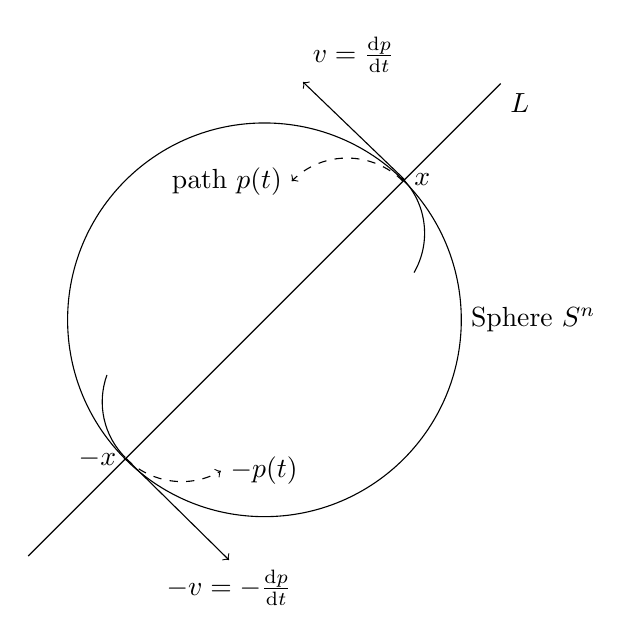
\begin{tikzpicture}
\draw (0,0) -- (6,6) node[anchor=north west] {$L$};
\draw (3,3) circle [radius=2.5] node[right=2.5cm]{Sphere $S^n$};
\draw (4.9,3.6) arc [start angle=-30, end angle=45, radius=1cm];
\draw[dashed, ->] (4.76,4.76) arc [start angle=45, end angle=135, radius=1cm]  node[anchor=east] {path $p(t)$};
\draw (1.0,2.3) arc [start angle=160, end angle=225, radius=1cm];
\draw[dashed, ->] (1.24,1.24) node[anchor=east] {$-x$} arc [start angle=225, end angle=300, radius=1cm] node[anchor=west] {$-p(t)$};
\draw[->] (1.24,1.24) -- (2.55,-0.05) node[anchor=north] {$-v=-\frac{\mathrm{d}p}{\mathrm{d}t}$};
\draw[->] (4.78,4.78) node[anchor=west] {$x$} -- (3.49,6.02) node[anchor=south west]  {$v=\frac{\mathrm{d}p}{\mathrm{d}t}$};
\end{tikzpicture}
\caption{}
\end{figure}
But each such pair determines, and is determined by, a linear mapping
\[
\ell: \mathrm{L} \varrightarrow{} \mathrm{L}^{\perp},
\]
where
\[
\ell(x)=v.
\]
Thus the tangent space of $\projective^{n}$ at $\{\pm x\}$ is canonically isomorphic to the vector space $\Hom(L, L^{\perp})$. It follows that the tangent vector bundle $\tau$ is canonically isomorphic to the bundle $\Hom(\tautological_n^1, \tautological^{\perp})$. This completes the proof of Lemma \ref{lem:04.04}.

\end{proof}

We cannot compute $\sw(\projective^n)$ directly from this lemma since we do not yet have any procedure for relating the Stiefel-Whitney classes of $\Hom(\tautological_n^1, \tautological^{\perp})$ to those of $\tautological_n^1$ and $\tautological^{\perp}$. However the computation can be carried through as follows. Let $\trivialbundle^1$ be a trivial line bundle over $\projective^{n}$.

\begin{theorem}
\label{thm:04.05}
The Whitney sum $\tau \oplus \trivialbundle^{1}$ is isomorphic to the $(n+1)$-fold Whitney sum $\tautological_{n}^{1} \oplus \tautological_{n}^{1} \oplus \ldots \oplus \tautological_{n}^{1}$. Hence the total Stiefel-Whitney class of $\projective^{n}$ is given by\index{binomial coefficients}
\[
\sw(\projective^{n})=(1+a)^{n+1}=1+\binom{n+1}{1}a + \binom{n+1}{2}a^2 + \dots + \binom{n+1}{n}a^{n} .
\]
\end{theorem}

\begin{proof}
The bundle $\Hom(\tautological_{n}^{1}, \tautological_{n}^{1})$ \index{Hom}\index{trivial bundle $\trivialbundle^n$} is trivial since it is a line bundle with a canonical nowhere zero cross-section. Therefore
\[
\tau \oplus \trivialbundle^{1} \cong \Hom(\tautological_{n}^{1}, \tautological^{\perp}) \oplus \Hom(\tautological_{n}^{1}, \tautological_{n}^{1}) .
\]
This is clearly isomorphic to
\[
\Hom(\tautological_{n}^{1}, \tautological^{\perp} \oplus \tautological_{n}^{1}) \cong \Hom(\tautological_{n}^{1}, \trivialbundle^{n+1}),
\]
and therefore is isomorphic to the $(n+1)$-fold sum
\[
\Hom(\tautological_{n}^{1}, \trivialbundle^{1} \oplus \ldots \oplus \trivialbundle^{1}) \cong \Hom(\tautological_{n}^{1}, \trivialbundle^{1}) \oplus \ldots \oplus \Hom(\tautological_{n}^{1}, \trivialbundle^{1})
\]
But the bundle $\Hom(\tautological_{n}^{1}, \trivialbundle^{1})$ is isomorphic to $\tautological_{n}^{1}, \operatorname{since} \tautological_{n}^{1}$ has a Euclidean metric. (Compare Problem \ref{prob-3-D}.) This proves that
\[
\tau \oplus \trivialbundle^{1} \cong \tautological_{n}^{1} \oplus \ldots \oplus \tautological_{n}^{1}
\]
Now the Whitney product theorem\index{Whitney product theorem} (Axiom~\ref{axi:04.03}) implies that $\sw(\tau)=\sw(\tau \oplus \trivialbundle^{1})$ is equal to
\[
\sw(\tautological_{n}^{1}) \ldots \sw(\tautological_{n}^{1})=(1+a)^{n+1}
\]
Expanding by the binomial theorem, this completes the proof of \ref{thm:04.05}.

\end{proof}

Here is a table of the binomial coefficients $\binom{n+1}{i}$ modulo 2 , for $n \leq 14$.

{
\newcommand{\hs}{\hspace{7pt}}
$
\begin{array}{lc}
         & 1 \\
         & 1 \hs 1 \\
 P^1:    & 1 \hs 0 \hs 1 \\
 P^2:    & 1 \hs 1 \hs 1 \hs 1 \\
 P^3:    & 1 \hs 0 \hs 0 \hs 0 \hs 1 \\
 P^4:    & 1 \hs 1 \hs 0 \hs 0 \hs 1 \hs 1 \\
 P^5:    & 1 \hs 0 \hs 1 \hs 0 \hs 1 \hs 0 \hs 1 \\
 P^6:    & 1 \hs 1 \hs 1 \hs 1 \hs 1 \hs 1 \hs 1 \hs 1 \\
 P^7:    & 1 \hs 0 \hs 0 \hs 0 \hs 0 \hs 0 \hs 0 \hs 0 \hs 1 \\
 P^8:    & 1 \hs 1 \hs 0 \hs 0 \hs 0 \hs 0 \hs 0 \hs 0 \hs 1 \hs 1 \\
 P^9:    & 1 \hs 0 \hs 1 \hs 0 \hs 0 \hs 0 \hs 0 \hs 0 \hs 1 \hs 0 \hs 1 \\
 P^{10}: & 1 \hs 1 \hs 1 \hs 1 \hs 0 \hs 0 \hs 0 \hs 0 \hs 1 \hs 1 \hs 1 \hs 1 \\
 P^{11}: & 1 \hs 0 \hs 0 \hs 0 \hs 1 \hs 0 \hs 0 \hs 0 \hs 1 \hs 0 \hs 0 \hs 0 \hs 1 \\
 P^{12}: & 1 \hs 1 \hs 0 \hs 0 \hs 1 \hs 1 \hs 0 \hs 0 \hs 1 \hs 1 \hs 0 \hs 0 \hs 1 \hs 1 \\
 P^{13}: & 1 \hs 0 \hs 1 \hs 0 \hs 1 \hs 0 \hs 1 \hs 0 \hs 1 \hs 0 \hs 1 \hs 0 \hs 1 \hs 0 \hs 1 \\
 P^{14}: & 1 \hs 1 \hs 1 \hs 1 \hs 1 \hs 1 \hs 1 \hs 1 \hs 1 \hs 1 \hs 1 \hs 1 \hs 1 \hs 1 \hs 1 \hs 1 \\
\end{array}
$
}
\phantom{,}\newline\phantom{,}\newline
The right hand edge of this triangle can be ignored for our purposes since $\homology^{n+1}(\projective^{n}; \mathbb{Z} / 2)=0$. As examples one has:
\[
\begin{aligned}
&\sw(\projective^{2})=1+a+a^{2} \\
&\sw(\projective^{3})=1
\end{aligned}
\]
and
\[
\begin{aligned}
\sw(\projective^{4})=1+a+a^{4}.
\end{aligned}
\]
\begin{corollary} (Stiefel).
 The class $\sw(\projective^{n})$ is equal to 1 if and only if $n+1$ is a power of 2. Thus the only projective spaces which can be parallelizable are $\projective^{1}, \projective^{3}, \projective^{7}, \projective^{15}, \ldots .$
\end{corollary}

(We will see in a moment that $\projective^{1}, \projective^{3}$, and $\projective^{7}$ actually are parallelizable. On the other hand it is known that the higher projective spaces $\projective^{15}, \projective^{31}, \ldots$ are not parallelizable. See \cite{bott-milnor1958},\cite{kervaire1958},\cite{adams1960}.) \label{problems page 47} %needed for ch11 --deri
\begin{proof}
The identity $(a+b)^{2} \equiv a^{2}+b^{2}$ modulo 2 implies that
\[
(1+a)^{2^{r}}=1+a^{2^{r}}
\]
Therefore if $n+1=2^{r}$ then
\[
\sw(\projective^{n})=(1+a)^{n+1}=1+a^{n+1}=1 .
\]
Conversely if $n+1=2^{r} m$ with $m$ odd, $m>1$, then

\[
 \sw(P^{n})=(1+a)^{n+1}=(1+a^{2^{r}})^{m}  =1+m a^{2^{r}}+\frac{m(m-1)}{2} a^{2 \cdot 2^{r}}+\ldots \neq 1
\]

since $2^{r}<n+1$. This completes the proof.
\end{proof}

\end{document}